\documentclass[11pt]{article}

\usepackage{mathptmx}
\usepackage{url}
\usepackage{graphicx}
\graphicspath{{images/}}

\newcommand*{\ls}{\textsc{LearnSAT}}
\newcommand*{\pl}{\textsc{Prolog}}
\newcommand*{\sw}{\textsc{SWI-Prolog}}
\newcommand*{\dt}{\textsc{dot}}

\textwidth=15cm
\textheight=21cm
\topmargin=0pt
\headheight=0pt
\oddsidemargin=5mm
\headsep=0pt
\renewcommand{\baselinestretch}{1.1}
\setlength{\parskip}{0.20\baselineskip plus 1pt minus 1pt}
\parindent=0pt


\begin{document}

\thispagestyle{empty}

\begin{center}

\textbf{\LARGE \ls{}: A SAT Solver for Education}

\bigskip

\textbf{\Large Moti Ben-Ari}

\bigskip

\large\url{http: //www.weizmann.ac.il/sci-tea/benari/}

\end{center}

\begin{center}
\copyright{} 2017 by Moti Ben-Ari.
\end{center}
{\footnotesize This work is licensed under the Creative Commons Attribution-ShareAlike 3.0
License. To view a copy of this license, visit
\url{http://creativecommons.org/licenses/by-sa/3.0/}; or, (b) send a letter
to Creative Commons, 543 Howard Street, 5th Floor, San Francisco,
California, 94105, USA.}


\section{Introduction}

A SAT solver is a program that searches for an assignment of truth values to the atoms of a propositional formula in conjunctive normal form (CNF) that satisfies the formula \cite[Chapter~6]{mlcs}. If no such assignment exists, the SAT solver will report that the formula is unsatisfiable. Since all $\mathcal{NP}$-complete problems can be encoded in a CNF formula and the encoding is relatively simple to perform, an efficient implementation of SAT solving can be applied to find solutions to many practical problems. For this reason, Donald Knuth calls SAT solvers a ``killer app'' \cite{knuth-sat}. 

The literature on SAT solving is extensive: the \emph{Handbook of Satisfiability} \cite{SAT} of almost one thousand pages covers theory, algorithms and applications, and Knuth's 300-page Section~7.2.2.2 contains over 500 exercises \cite{knuth-sat}. Since SAT solvers are widely used, it is essential that quality learning materials be available for students, even those who do not intend to become researchers, for example, undergraduate students taking a course in mathematical logic. Such learning materials will also be helpful for people using SAT solvers in applications. Instructors should be enabled to create learning materials that demonstrate the central algorithms in detail.

\ls{} is a SAT solver designed for educational use according to the following criteria:

\begin{itemize}
\item A detailed trace of the algorithm's execution is displayed. Its content can be set by the user.

\item Implication graphs and assignment trees are generated automatically.

\item The implementation is concise, easy to understand and well documented. 

\item The software is easy to install and use.

\item The input to the program is a formula in clausal form written in a
readable symbolic form. Programs to convert to and from DIMACS format are provided.

\item SAT solving is explained in a detailed tutorial and many example programs are provided.
\end{itemize}


\section{The \ls{} SAT solver}

\ls{} implements the core algorithms of many modern SAT
solvers: DPLL with conflict-driven clause learning (CDCL) and
non-chro\-no\-log\-i\-cal backtracking (NCB). \ls{} can be
run in three modes---plain DPLL, DPLL with CDCL, and DPLL with both CDCL
and NCB---so that the student can examine the improvements obtained by
each refinement. CDCL is implemented by backwards resolution from a conflict
clause to a unique implication point (UIP). It is also possible to
compute dominators in the implication graph although this computation is
just displayed and not used. The user can specify the order in which literals are assigned. In addition, two heuristics for lookahead can be selected.

\section{The output of \ls{}}

The key to learning sophisticated algorithms like SAT solving is a trace
of the step-by-step execution of the algorithm. The user of
\ls{} can choose \emph{any} subset of 24 display options in
order to tailor the output to a specific learning context. The display
options include elementary steps like decision assignments, unit
propagations and identifying conflict clauses, as well as the advanced steps of
CDCL: the resolution steps used to obtained a learned clause and the
search for UIPs. The Appendix shows the (default) output for the example
in \cite{mlm} run in NCB mode.

\ls{} can generate two types of graphs that are rendered using the \textsc{dot} tool: trees showing the search through the assignments  (Figure~\ref{fig.1}) and implication graphs that display the process for learning clauses from conflicts  (Figure~\ref{fig.2}). These graphs incrementally.

\begin{figure}
\vspace*{-2ex}
\begin{center}
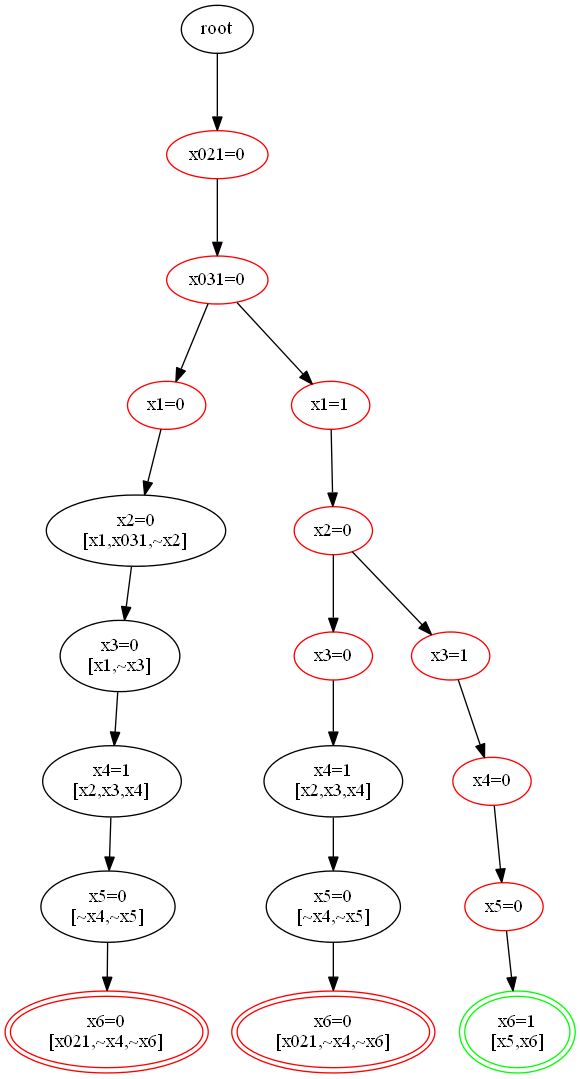
\includegraphics[keepaspectratio=true,height=.6\textheight]{tree1-color}
\caption{Assignment tree for DPLL mode}\label{fig.1}
\end{center}
\end{figure}
 
\begin{figure}
\vspace*{-2ex}
\begin{center}
\includegraphics[keepaspectratio=true,width=\textwidth]{graph-color}
\caption{Implication graph for CDCL mode}\label{fig.2}
\end{center}
\end{figure}

\section{Examples}

The \ls{} archive includes the examples used in \cite{mz,mlm,ms} to help students read these articles. The archive includes encodings of the following problems:
\begin{itemize}
\item Graphical combinatorics: graph coloring, Tseitin graphs.
\item Games: Sudoku, $4$-queens, colored queens.
\item Number theory: Ramsey theory, Schur triples, Langford's and van der Waerden's problems.
\item Constrained arrangements: pebbling formulas, seating guests at a table.
\item Bounded model checking.
\end{itemize}

\newpage

The list of clauses for the 2-hole pigeonhole problem is:
\begin{small}
\begin{verbatim}
hole2 :- dpll([
  [p11, p12],   [p21, p22],   [p31, p32],     % Each pigeon in hole 1 or 2
  [~p11, ~p21], [~p11, ~p31], [~p21, ~p31],   % No pair is in hole 1
  [~p12, ~p22], [~p12, ~p32], [~p22, ~p32],   % No pair is in hole 2
  ], _).
\end{verbatim}
\end{small}

\section{Implementation}

\ls{} is implemented in \pl{} which was chosen because \pl{} programs are extremely concise: the core algorithms take only about 250 lines. The \sw{} compiler was used: it is available for the systems used by students, such as Windows and Mac. It is easy to install and has a comprehensive reference manual.

\section{Documents}

\LaTeX{} and PDF files are provided for the \ls{} User's Guide and Software Documentation and the \ls{} Tutorial.

\bibliographystyle{plain}
\bibliography{learnsat}

\newpage

\appendix
\section{Output for the example in \cite{mlm}}
\begin{small}
\begin{verbatim}
LearnSAT (version 2.0)
Decision assignment: x021=0@1
Decision assignment: x031=0@2
Decision assignment: x1=0@3
Propagate unit: ~x2 derived from: 1. [x1,x031,~x2]
Propagate unit: ~x3 derived from: 2. [x1,~x3]
Propagate unit: x4 derived from: 3. [x2,x3,x4]
Propagate unit: ~x5 derived from: 4. [~x4,~x5]
Propagate unit: ~x6 derived from: 5. [x021,~x4,~x6]
Conflict clause: 6. [x5,x6]
Not a UIP: two literals are assigned at level: 3
Clause: [x5,x6] unsatisfied
Complement of: x5 assigned true in the unit clause: [~x4,~x5]
Resolvent of the two clauses: [x6,~x4] is also unsatisfiable
Not a UIP: two literals are assigned at level: 3
Clause: [x6,~x4] unsatisfied
Complement of: x6 assigned true in the unit clause: [x021,~x4,~x6]
Resolvent of the two clauses: [x021,~x4] is also unsatisfiable
UIP: one literal is assigned at level: 3
Learned clause: [x021,~x4]
Non-chronological backtracking to level: 1
Skip decision assignment: x1=1@3
Skip decision assignment: x031=1@2
Decision assignment: x021=1@1
Decision assignment: x031=0@2
Decision assignment: x1=0@3
Propagate unit: ~x2 derived from: 1. [x1,x031,~x2]
Propagate unit: ~x3 derived from: 2. [x1,~x3]
Propagate unit: x4 derived from: 3. [x2,x3,x4]
Propagate unit: ~x5 derived from: 4. [~x4,~x5]
Propagate unit: x6 derived from: 6. [x5,x6]
Satisfying assignments:
[x021=1@1,x031=0@2,x1=0@3,x2=0@3, x3=0@3,x4=1@3,x5=0@3,x6=1@3]
Statistics: clauses=6,variables=8,units=10,decisions=6,conflicts=1
\end{verbatim}
\end{small}
\end{document}
